\documentclass[math-font=newcm]{sjtuarticle}

% \usepackage[hybrid,citations,fencedCode,underscores=false]{markdown}

\usepackage[style=gb7714-2015]{biblatex}
\addbibresource{ref.bib}

\graphicspath{{figs/}}

\usepackage{float}

\def\dd{\mathrm{d}}

\usepackage{listings}
\captionsetup[lstlisting]{labelfont=bf,justification=justified}
\providecommand{\linkcode}[1]{\href{run:../source/#1}{#1}}
\providecommand{\code}[2]{\lstinputlisting[language=#2,caption=\href{run:#1}{\ttfamily #1}]{#1}}
\providecommand{\codeRange}[4]{\lstinputlisting[language=#2,caption=\href{run:#1}{\ttfamily #1},firstline=#3,lastline=#4]{#1}}
\definecolor{grey}{rgb}{0.8,0.8,0.8}
\definecolor{darkgreen}{rgb}{0,0.3,0}
\definecolor{darkblue}{rgb}{0,0,0.3}
\lstset{%
    numbers=left, %行号
    numberstyle=\tiny\color{grey},
    showstringspaces=false,
    showspaces=false,%
    tabsize=4,%
    frame=shadowbox,%
    basicstyle={\ttfamily\small},%
    keywordstyle=\color{blue!80!black}\bfseries,%
    identifierstyle=,%
    commentstyle=\color{green!50!blue}\itshape,%
    stringstyle=\color{green!50!black},%
    rulesepcolor=\color{gray!20!white},
    breaklines,
    columns=flexible,
    extendedchars=false,
    mathescape=true,
    escapebegin=\color{green!50!blue}
}

\usepackage[linesnumbered,ruled]{algorithm2e}
\usepackage[colorlinks]{hyperref}

\title{Shading Model: Local}
\author{Log Creative}
\date{2024 年 6 月 2 日}
\begin{document}
\maketitle

\tableofcontents*
\clearpage

\section{场景设置}

本项目设置了一个圆柱、一个多面体(立方体)、一个球体、一个圆锥、两个光源$m=2$。并额外实现了带材质的地板。实现了局部光照模型的环境、漫射、高光分量。

\section{光照模型}

本项目实现了冯氏光照模型(Phong Lighting Model),按下式计算每个片段的光照强度(包含颜色分量):

\begin{equation}\label{eq:phong}
    I_\lambda=I_{a\lambda}k_a+\sum_{1\leq i\leq m}S_i[k_dL_{d\lambda}(l\cdot n)+k_sL_{s\lambda}(r\cdot v)^n]\quad S_i=\frac{1}{a+bd_i+cd_i^2}
\end{equation}

\subsection{环境(ambient)}

环境分量为 $I_{a\lambda}k_a$,本项目中环境光照强度 $I_{a\lambda}=0.1$,材质的环境属性将与漫射属性相同,对于立方体的典型值为 $k_a=[1.0, 0.5, 0.31]$。

\subsection{漫射(diffuse)}
漫射分量为 $\sum_{1\leq i\leq m}S_ik_dL_{d\lambda}(l\cdot n)$。光源漫射强度 $L_{d\lambda}=0.8$,材质的漫射属性对于立方体的典型值为 $k_d=k_a=[1.0, 0.5, 0.31]$,而 $l\cdot n$ 对于每个片段都是不同的,反映了该片段的漫射照亮程度:$l$ 为光源位置向量与片段位置向量之间的向量差的单位向量,$n$ 为法向量,为了避免不等比缩放可能会导致的不垂直表面的问题\cite{normal},法向量的实际计算公式为 $(M^{-1})^\top n$,其中 $M$ 为模型(Model)矩阵。注意由于负数的光照是没有意义的,所以事实上会取与 0 的最大值,即 $\max(l\cdot n, 0)$。

\subsection{高光(specular)}
高光分量为 $\sum_{1\leq i\leq m}S_ik_sL_{s\lambda}(r\cdot v)^n$。光源高光属性 $L_{s\lambda}=1.0$,材质高光属性 $k_s=[0.5,0.5,0.5]$,而 $(r\cdot v)^n$ 会根据视角的不同发生变化:$r$ 为反射方向向量,为前文中光源方向向量 $l$ 以法向量 $n$ 为对称中镜像得到;$v$ 为视角方向向量,为视角位置向量与片段位置向量的向量差单位向量,当 $r$ 与 $v$ 的方向越重合,说明高光分量越大,注意由于负数的高光分量也是没有意义的,所以也会与 0 取最大值,即 $\max(r\cdot v,0)$。最后使用反光度(shiness)$n$进行乘幂,此处材质 $n=32$,地板$n=8$。

\subsection{衰减(attenuation)}
点光源随着光线传播距离的增长逐渐衰减,$S_i=\frac{1}{a+bd_i+cd_i^2}$ 即描绘了这种模型。为了使光源覆盖 50 的距离,根据文献 \parencite{light},本项目取常数项 $a=1.0$,一次项$b=0.09$,二次项$c=0.032$。注意本项目没有将环境分量算入衰减中,也就是严格按照公式 \eqref{eq:phong} 的计算方法。

\section{实现细节}

\subsection{运行环境}

主要的代码结构参考文献 \parencite{learnopengl},编译环境使用了基于CMake的跨平台代码库 \parencite{simpleopengl},包含 GLFW 3.4,GLAD 4.3(程序主体基于 OpenGL 3.3),并额外添加了 GLM 矩阵运算库 1.0.1 \cite{glm} 和图像加载库 stb\_image 2.29\cite{stb}。本项目提供了 Windows,macOS,Linux 等多个平台的预编译二进制文件。

\subsection{源代码结构}

源代码主要存放于 \href{run:../source/src/main.cpp}{src/main.cpp} 中,依赖于 \verb"Shader" 类\cite{shader} \href{run:../source/src/shader_m.h}{src/shader\_m.h} 和 \verb"Camera" 类\cite{camera} \href{run:../source/src/camera.h}{src/camera.h}。

着色器代码存放于 assets/shader/ 文件夹中,包含
\begin{itemize}
    \item \linkcode{assets/shader/vertexShader.glsl} 模型顶点着色器;
    \item \linkcode{assets/shader/fragmentShader.glsl} 模型片段着色器;
    \item \linkcode{assets/shader/lightCubeVertexShader.glsl} 光源方块顶点着色器;
    \item \linkcode{assets/shader/lightCubeFragmentShader.glsl} 光源方块片段着色器(仅为了显示光源位置);
    \item \linkcode{assets/shader/planeVertexShader.glsl} 平面顶点着色器;
    \item \linkcode{assets/shader/planeFragmentShader.glsl} 平面片段着色器(考虑材质贴图)。
\end{itemize}

\subsection{模型构建}

\subsubsection{立方体}

直接对6个面的12个三角形定义顶点情况,如图 \ref{fig:cube} 所示,最后以 \verb"GL_TRIANGLES" 模式渲染。

\begin{figure}[h]
    \centering
    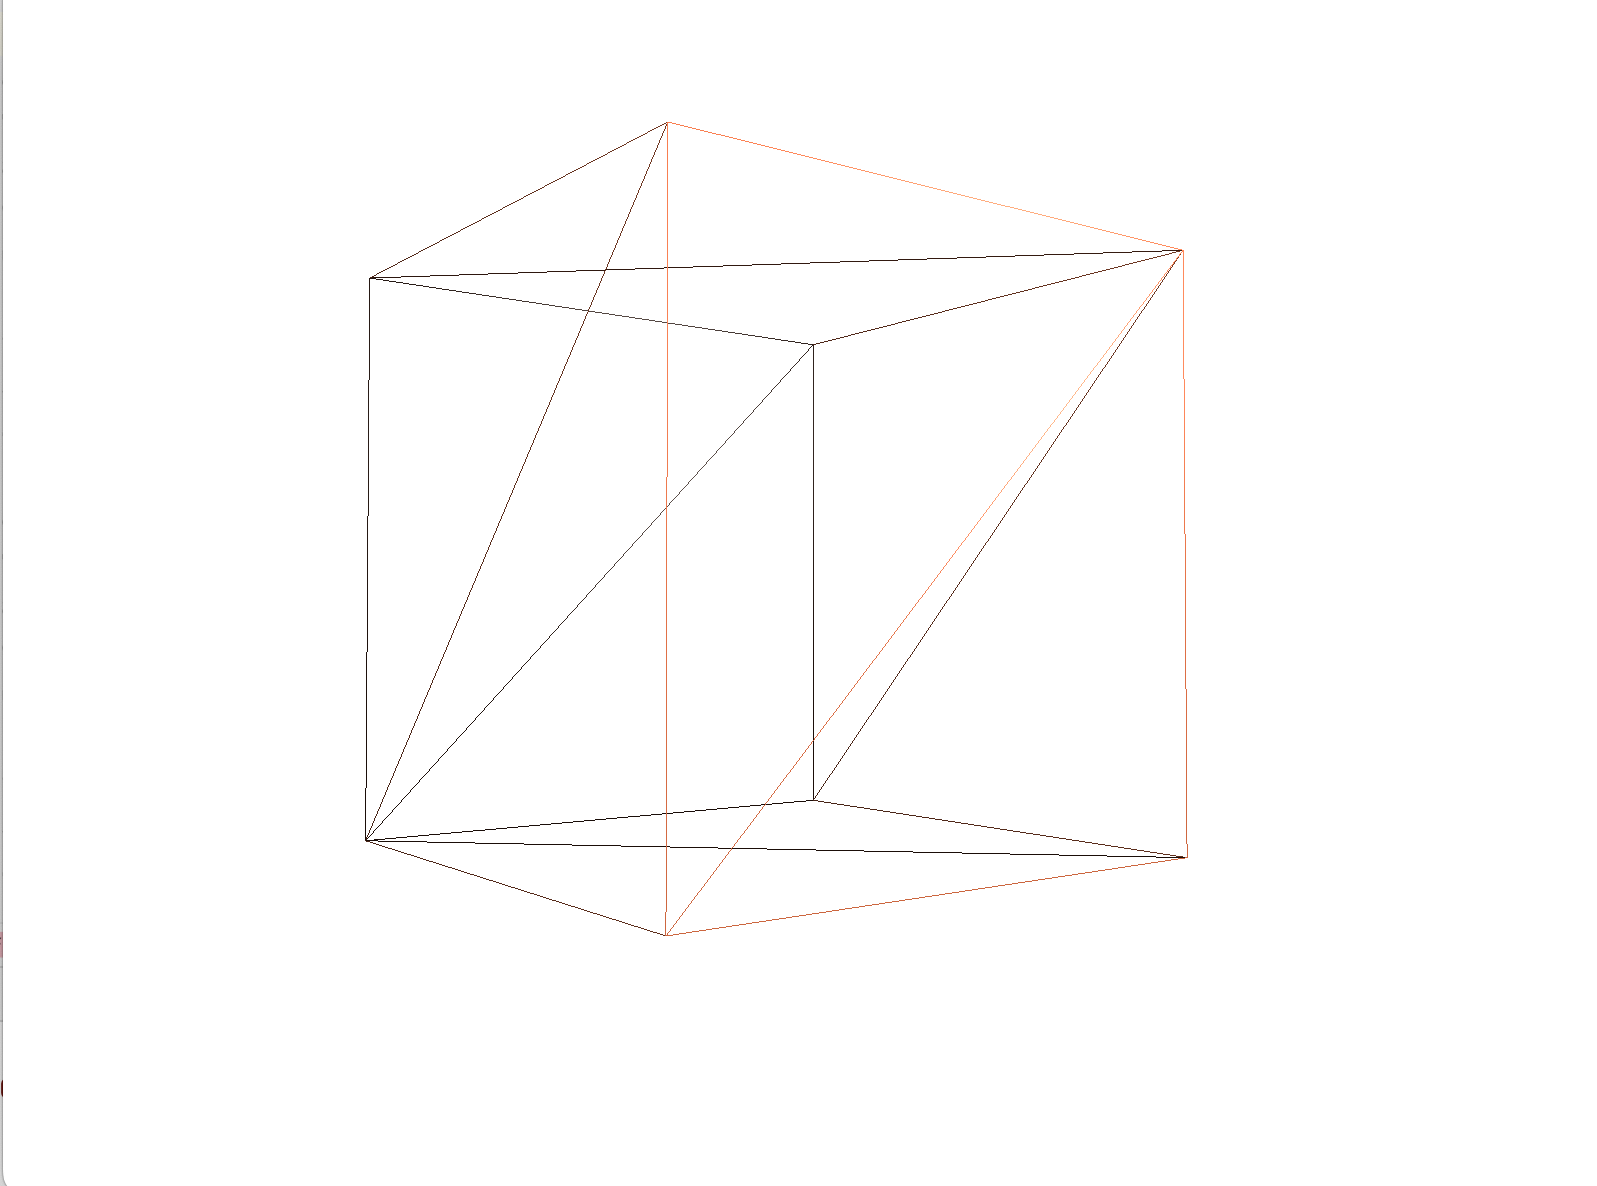
\includegraphics[width=0.5\textwidth]{cube.png}
    \caption{立方体线框模型}
    \label{fig:cube}
\end{figure}

\subsubsection{圆柱体}

圆柱体会定义圆周平均数 $N$,然后按照图 \ref{fig:cylinder} 所示的方法\cite{cylinder},首先画上下两个面,按 \verb"GL_TRIANGLE_FAN" 模式绘制,该模式要求先输入圆心,然后依次输入圆周上的点;然后画侧面,按 \verb"GL_TRIANGLE_STRIP" 模式绘制,不再使用 \verb"GL_TRIANGLES" 模式绘制的原因是可能会导致光照不均的三角侧面,如图 \ref{fig:wrongcy} 所示。

\begin{figure}[h]
    \begin{minipage}{0.45\textwidth}
        \centering
        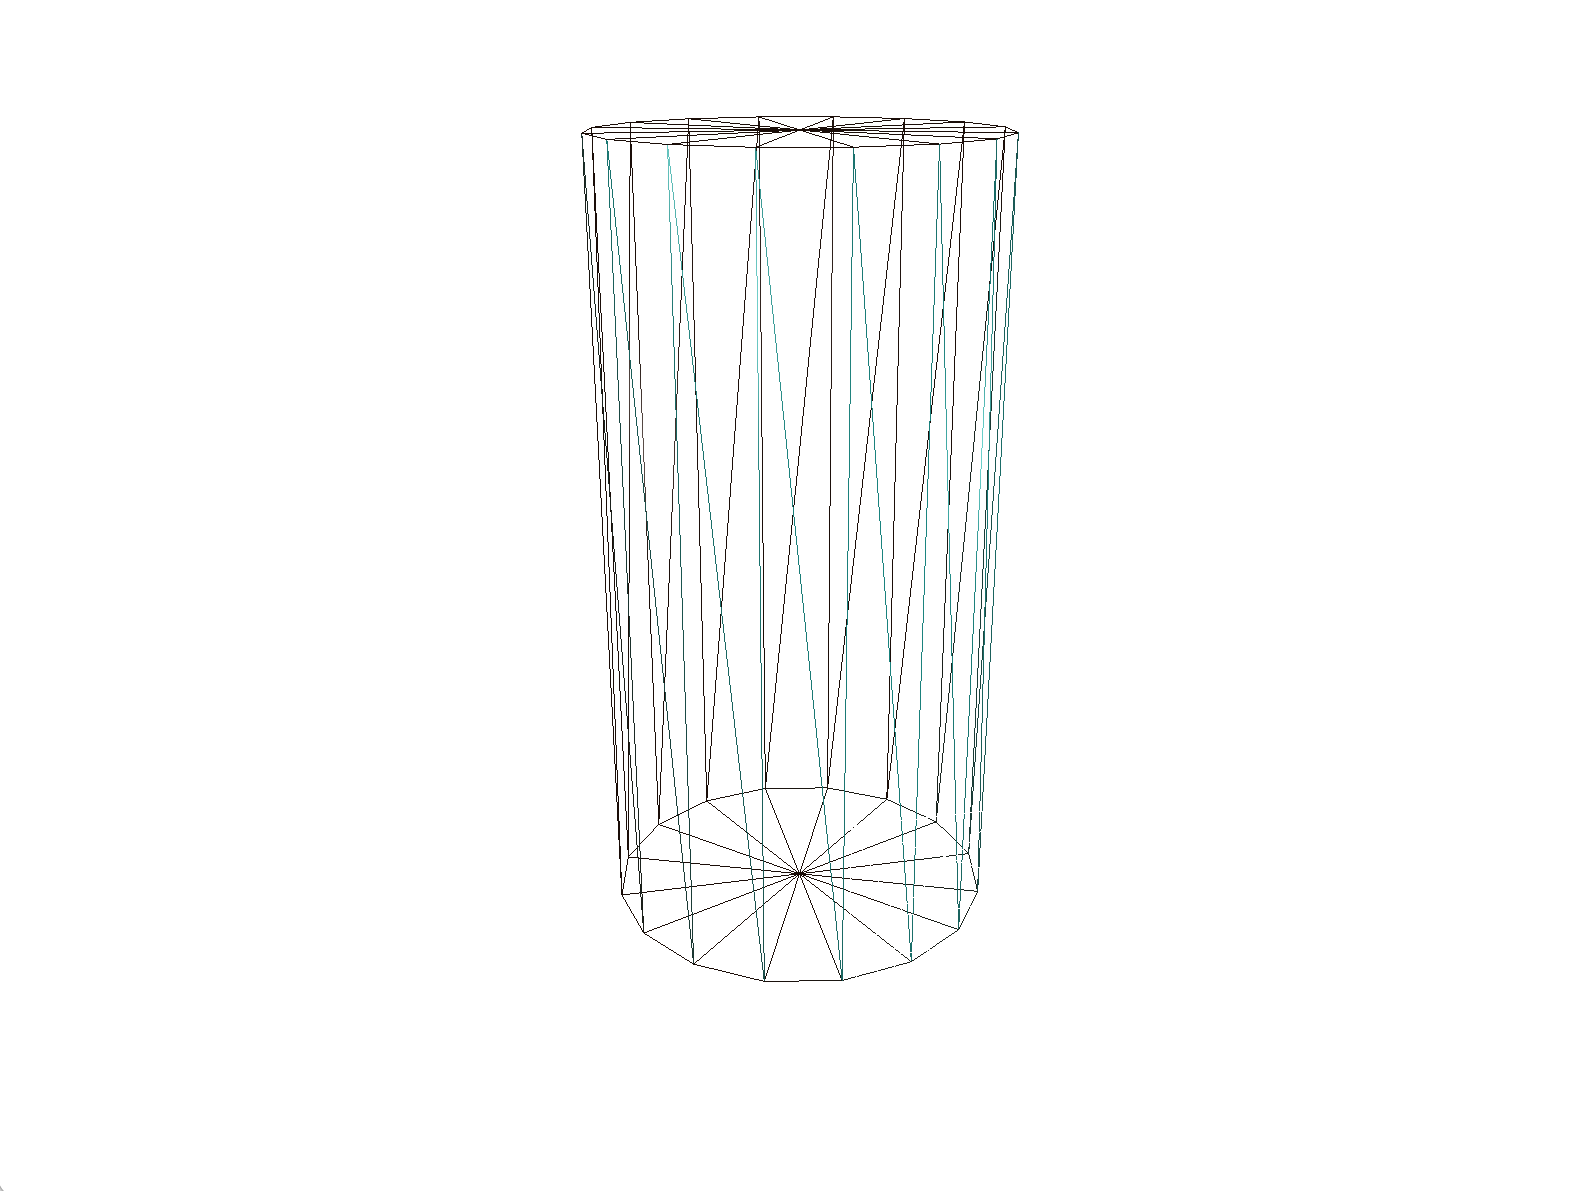
\includegraphics[width=0.9\textwidth]{cylinder.png}
        \caption{圆柱体线框模型}
        \label{fig:cylinder}
    \end{minipage}
    \begin{minipage}{0.45\textwidth}
        \centering
        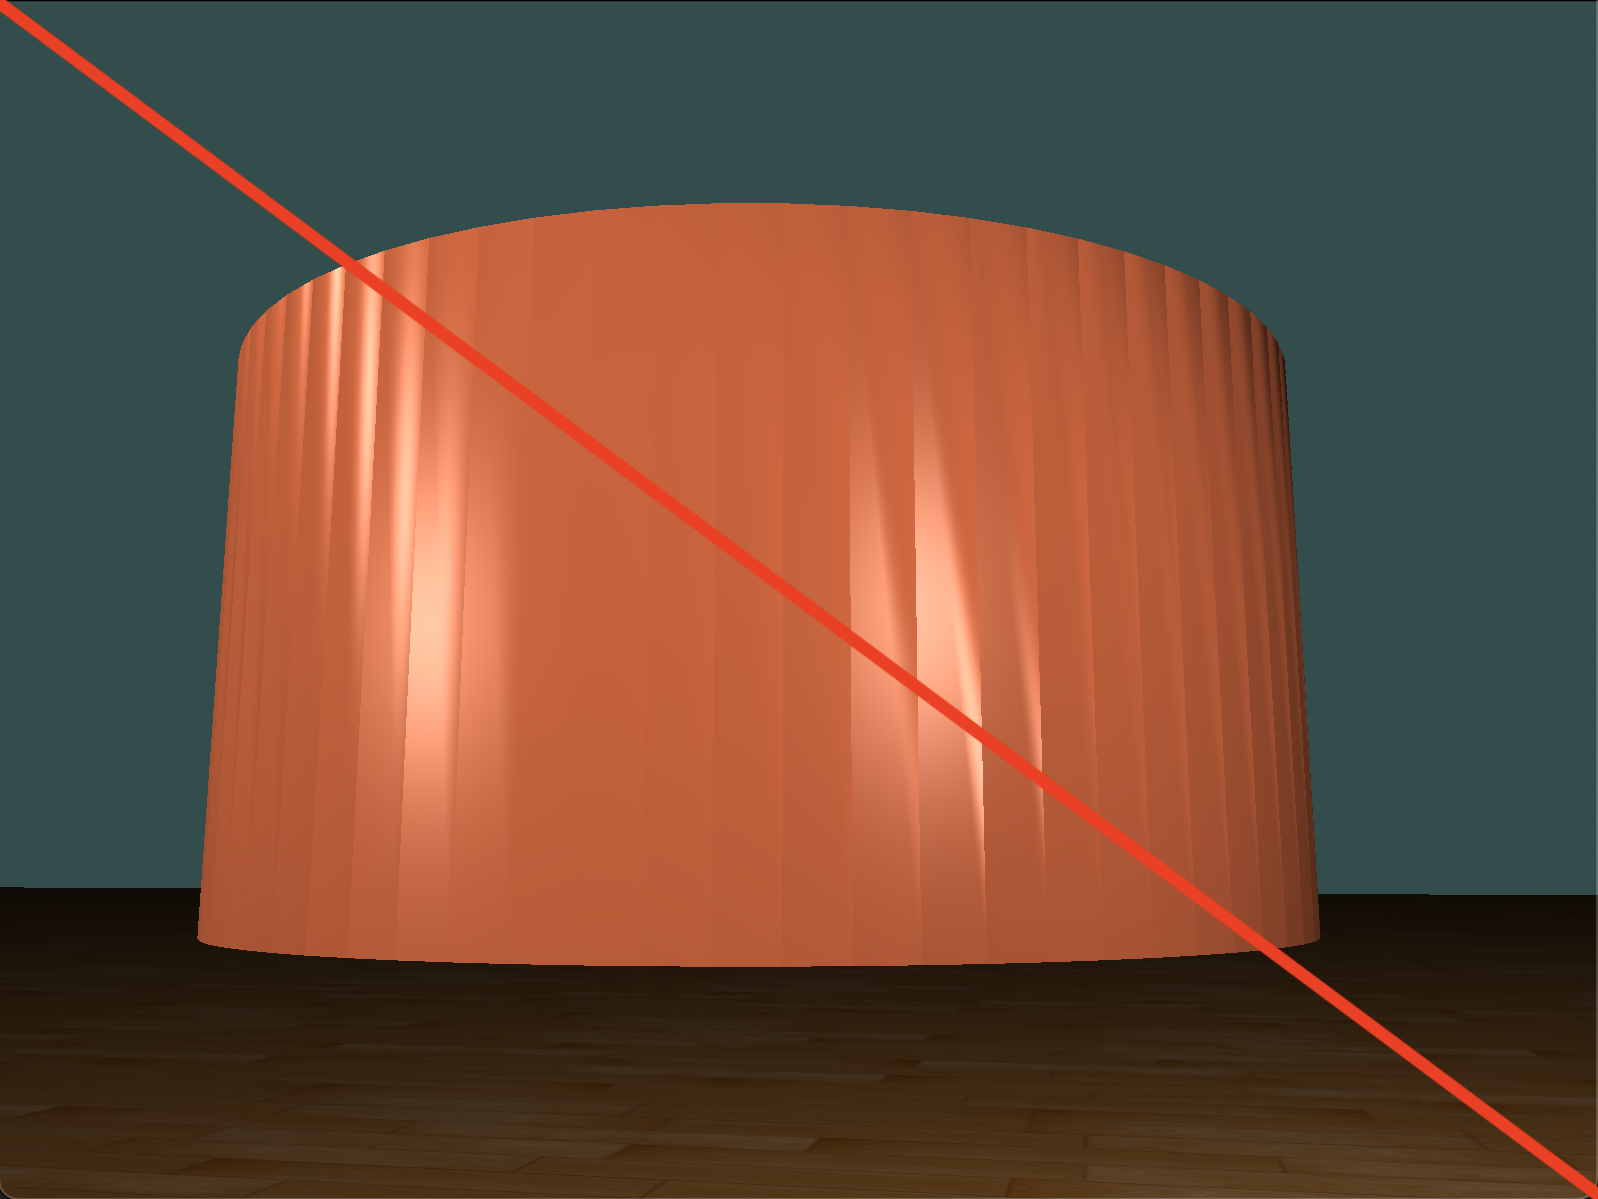
\includegraphics[width=0.9\textwidth]{wrongcy.png}
        \caption{错误的渲染方法}
        \label{fig:wrongcy}
    \end{minipage}
\end{figure}

\subsubsection{圆锥体}

圆锥体也会定义圆周平均数 $N$,然后按照图 \ref{fig:cone} 所示的方法,顶面和底面都按 \verb"GL_TRIANGLE_FAN" 模式绘制,只是顶面的圆心在 $(0,h,0)$ 处;底面的圆心在 $(0,0,0)$ 处。而侧面的法线计算如图 \ref{fig:conenorm} 所示,可见法线方向为 $(\cos\theta,\sin\theta,\frac{r}{h})$。

\begin{figure}[h]
    \begin{minipage}{0.45\textwidth}
        \centering
        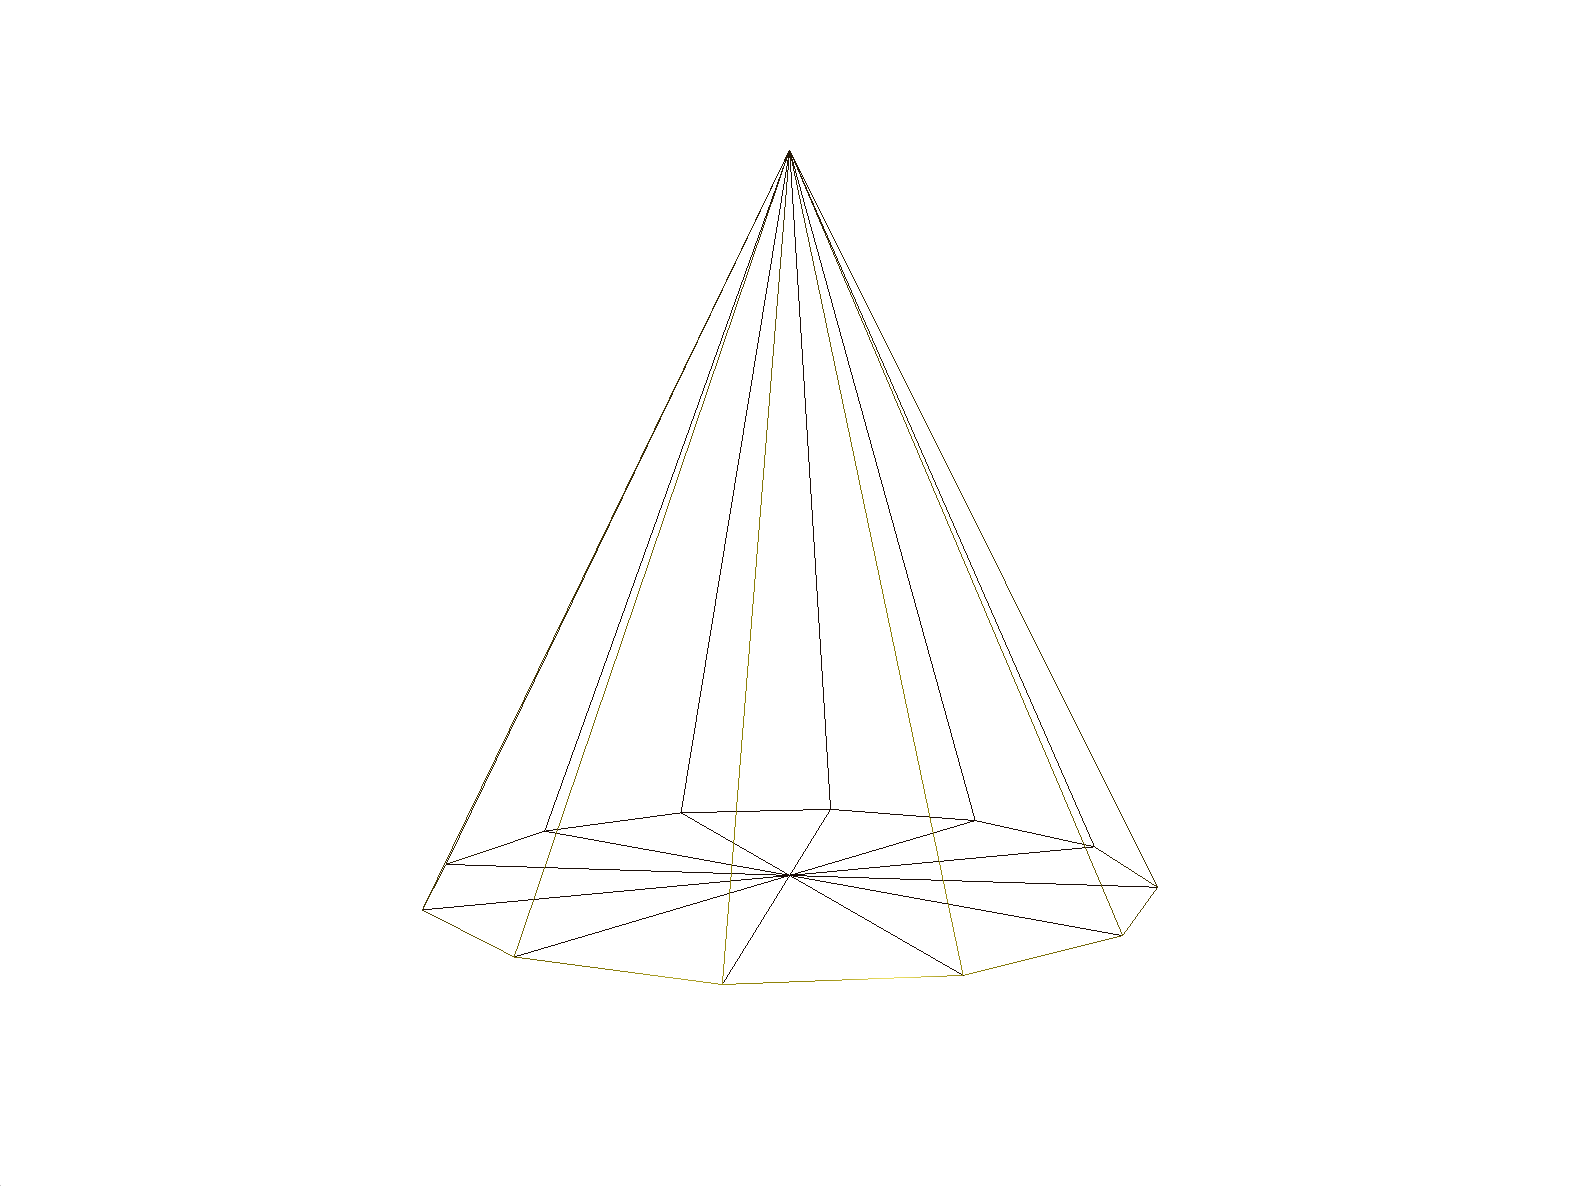
\includegraphics[width=0.9\textwidth]{cone.png}
        \caption{圆锥体线框模型}
        \label{fig:cone}
    \end{minipage}
    \begin{minipage}{0.45\textwidth}
        \centering
        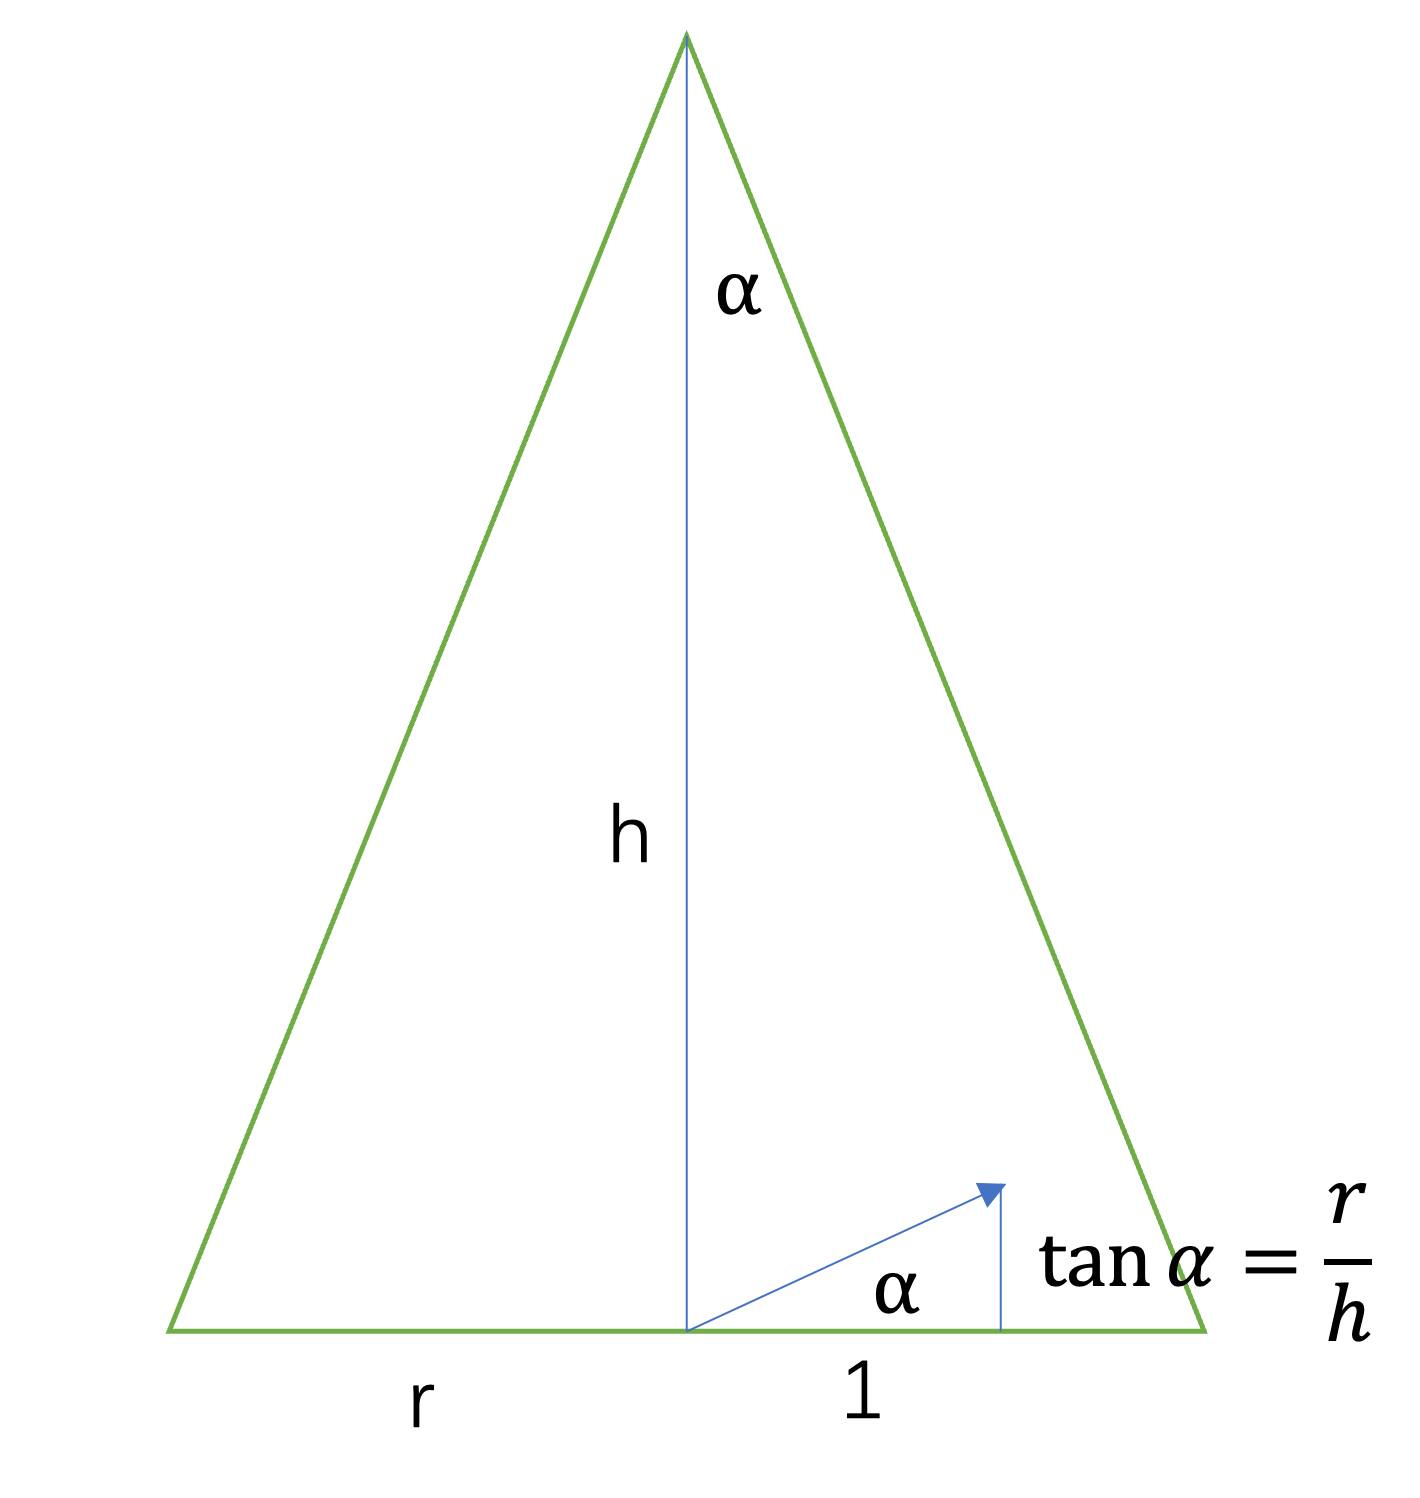
\includegraphics[width=0.6\textwidth]{conenorm.png}
        \caption{圆锥顶面的法线计算方法}
        \label{fig:conenorm}
    \end{minipage}
\end{figure}

\subsubsection{球体}

球体除了定义圆周平均数 $N$,还会定义纬度平均数 $M$,然后按照图 \ref{fig:sphere} 所示的方法,先按模式 \verb"GL_TRIANGLE_FAN" 绘制南北极,然后 \verb"GL_TRIANGLE_STRIP" 绘制侧面。按照球体的参数方程 \eqref{eq:sphere} 确定顶点位置。

\begin{equation}\label{eq:sphere}
    \begin{cases}
        x&=r\cos\theta\sin\phi\\
        y&=r\cos\phi\\
        z&=r\sin\theta\sin\phi
    \end{cases}\quad
    \begin{cases}
        n_x&=\cos\theta\sin\phi\\
        n_y&=\cos\phi\\
        n_z&=\sin\theta\sin\phi
    \end{cases}
\end{equation}

\begin{figure}[h]
    \centering
    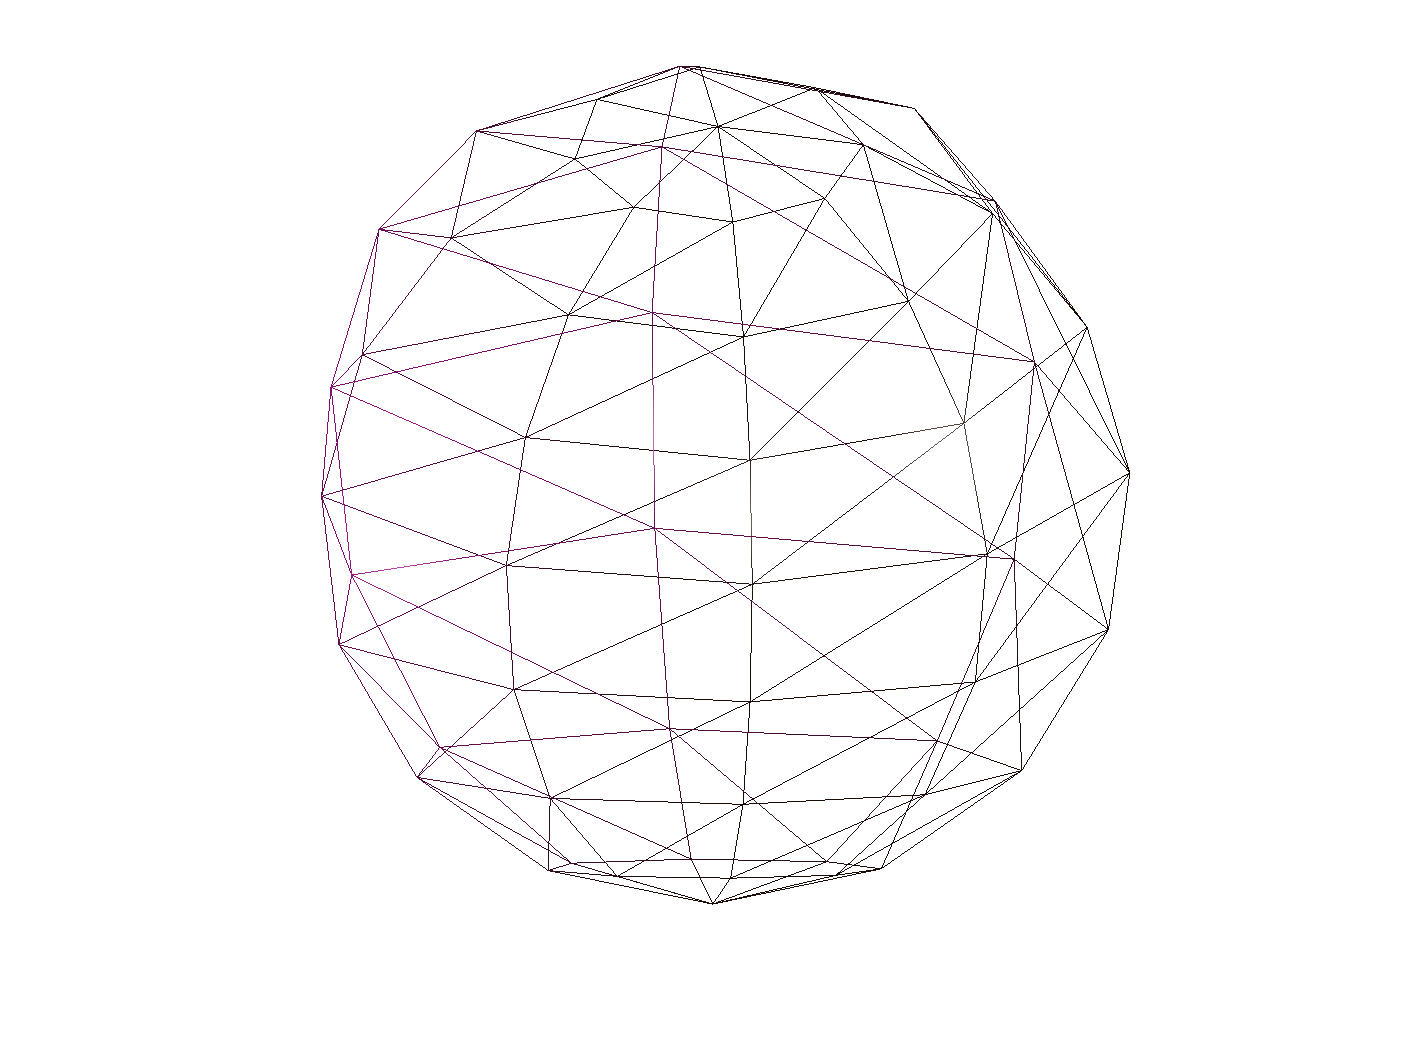
\includegraphics[width=0.5\textwidth]{sphere.png}
    \caption{球体线框模型}
    \label{fig:sphere}
\end{figure}

\subsection{多光源}

使用循环实现式 \eqref{eq:phong}。

\codeRange{../source/assets/shader/fragmentShader.glsl}{c}{55}{63}

\section{实验结果}

如图 \ref{fig:result} 所示,可以看到实验目标被很好的实现,几何模型被正确渲染,并实现了带材质的地板,他们都接受两个光的光照,基本每个模型上可以看到两个高光。还可以使用鼠标旋转视角,键盘 W A S D 移动摄像机位置,使用鼠标滚轮设定缩放。示例视频见 \linkcode{../video/demo.mp4},可执行文件位于 executables/ 文件夹。

\begin{figure}[h]
    \centering
    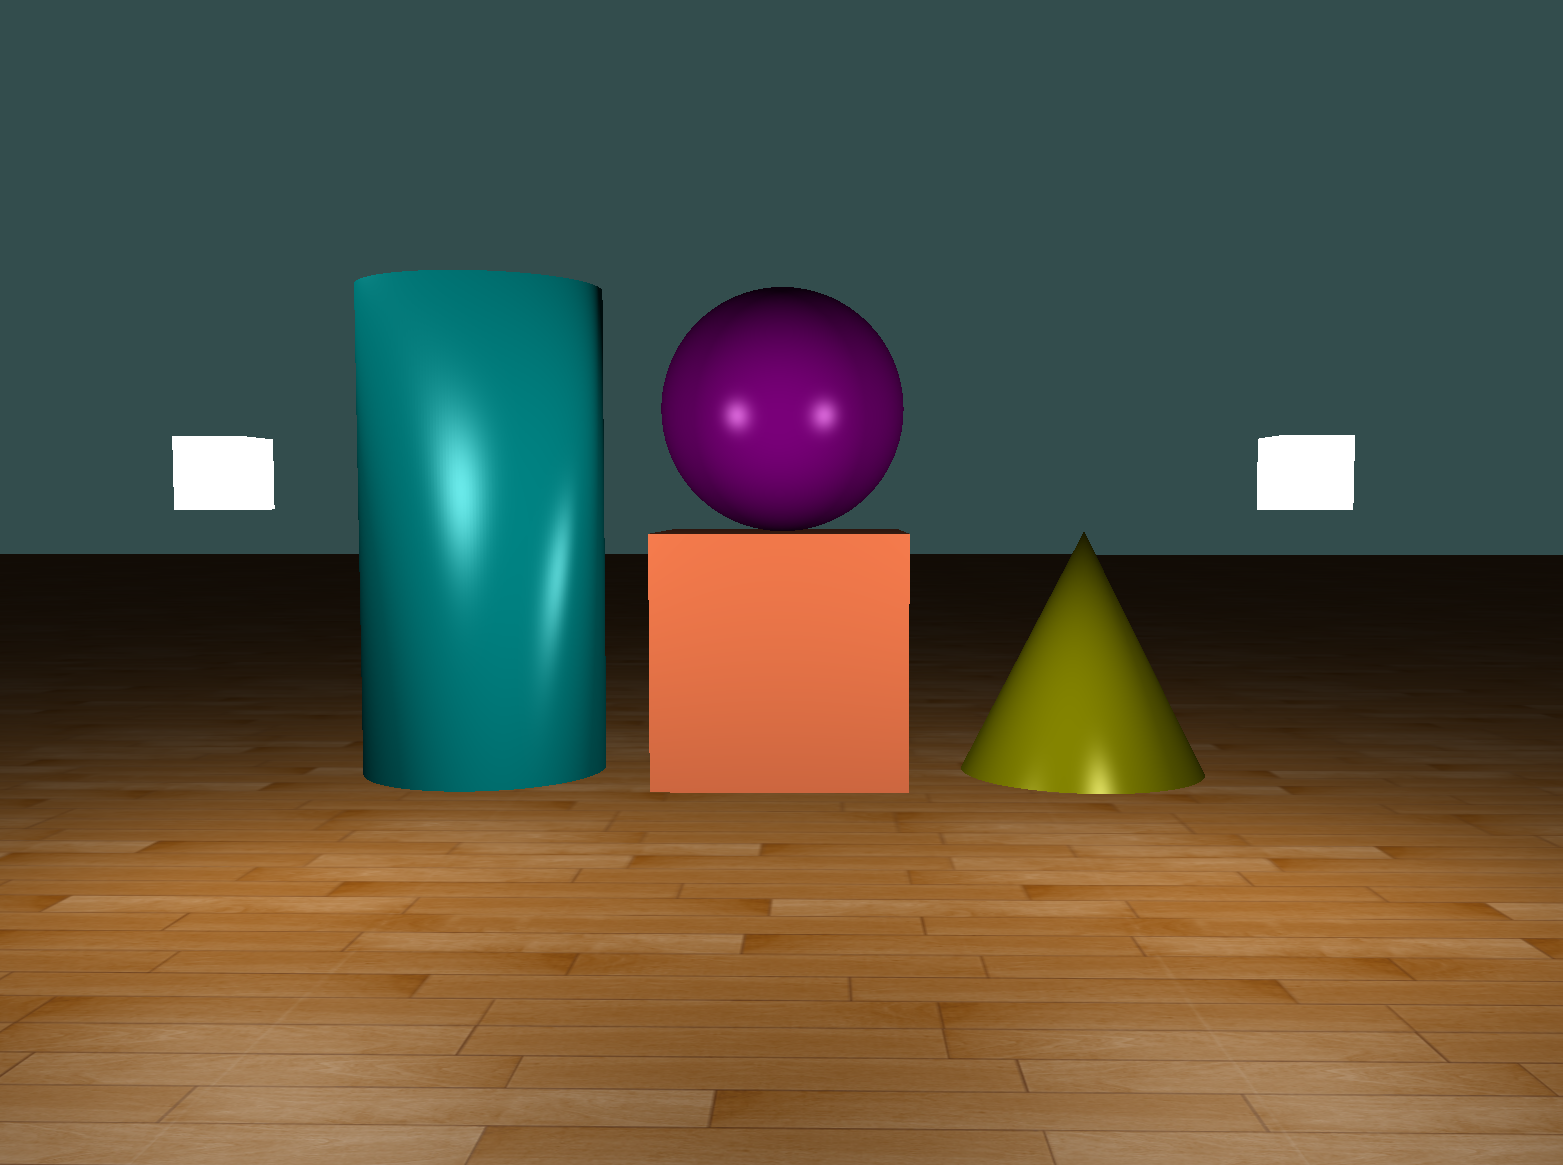
\includegraphics[width=0.5\textwidth]{result.png}
    \caption{实验结果}
    \label{fig:result}
\end{figure}

\printbibliography

\end{document}